\section{莫队算法}
\subsection{普通莫队}
\par \noindent 把整个区间 $[1,n]$ 分成若干块,以询问的左端点所在块为第一关键字,以询问的右端点大小为第二关键字,对询问进行排序,那么:
\begin{itemize}
\item 对于同一块的询问,$l$ 指针每次最多移动块的大小,$r$ 指针的移动则是单调的,总共移动最多 $n$ 。
\item 对于不同块的询问,$l$ 每次换块时最多移动两倍块的大小,$r$ 每次换块时最多移动 $n$ 。
\end{itemize}

\par \noindent \textbf{总结:}(用 $B$ 表示块的大小)$l$ 指针每次移动 $O(B)$,$r$ 指针每块移动 $O(n)$ 。
~\\
\par \noindent 所以:
\begin{itemize}
\item $l$ 的移动次数最多为询问数×块的大小,即 $O(mB)$ 。
\item $r$ 的移动次数最多为块的个数×总区间大小,即 $O(n^2/B)$ 。
\end{itemize}

\par \noindent 因此,总移动次数为 $O(mB+n^2/B)$ 。
~\\
\par \noindent 前两步先扩大区间(l-- 或 r++ ),后两步再缩小区间(l++ 或 r--)
\begin{minted}{c++}
int unit;  // 块的大小
struct Node {
  int l, r, id;
  bool operator<(const Node &x) const {
    if (l / unit != x.l / unit) return l < x.l;
    if ((l / unit) & 1)
      return r < x.r;  // 奇偶分组
    return r > x.r;
  }
};
// 前两步先扩大区间(`l--` 或 `r++`),后两步再缩小区间(`l++` 或 `r--`)
int main() {
    while (l > q[i].l) add(--l);
    while (r < q[i].r) add(++r);
    while (l < q[i].l) del(l++);
    while (r > q[i].r) del(r--);
}
\end{minted}
\subsection{树上莫队}
~\\
\par \noindent 欧拉序就是 DFS 序的升级版,在每一次遍历到这个节点的时候记录一次,离开这个节点的时候再记录一次。
~\\
\par \noindent 一般采用 $fir_x$ 表示 $x$ 在欧拉序中第一个出现的位置, $l a s_x$ 表示 $x$ 在欧拉序中第二个 (最后一个) 出现 的位置。
~\\
\par \noindent 当一个询问询问路径 $x \rightarrow y$ 的时候,如果 $x, y$ 在一条链上,询问的区间就是 $[f i r_x, f i r_y]$ ,否则就是 $[l a s_x,fir_y]$ ,具体询问区间可以使用 LCA 判断。
~\\
\par \noindent 需要注意的是当询问 $\left[l a s_x, f i r_y\right]$ 的时候,不能忘记计算他们 LCA 的贡献。
~\\
\par \noindent 由于一个点在欧拉序中会出现两次,因此树上莫队的修改采用奇增偶删原则,即若这个点是奇数次被修改就增加,偶数次被修改就减少。
\begin{minted}{c++}
void Work(int x) {
    vis[x] ^= 1;
    // 奇增偶删
    vis[x] ? Add(x) : Del(x);
}
int main () {
    sort(q + 1, q + m + 1, cmp);
    int l = 1, r = 0;
    for (int i = 1; i <= m; ++i)
    {
        while (l > q[i].l) Work(Eular[--l]);
        while (r < q[i].r) Work(Eular[++r]);
        while (l < q[i].l) Work(Eular[l++]);
        while (r > q[i].r) Work(Eular[r--]);
        if (q[i].lca) Work(q[i].lca);
        ans[q[i].id] = Ask(q[i].l, q[i].r);
        if (q[i].lca) Work(q[i].lca);
    }
    return 0;
}
\end{minted}

\subsection{值域分块}

\par \noindent 考虑一下莫队的本质,即莫队的复杂度分析,本质上分析的是 $l, r$ 移动的复杂度,也就是修改的复杂度。
~\\
\par \noindent 所以莫队可以本质上看成一个 $O(mB+n^2/B)$ 修改,$O(m)$ 询问的数据结构。观察到询问数较少,于是可以用一个可以快速修改,低速查询的 ds 来维护值域。
~\\
\par \noindent 自然就是值域分块:需要一个值域上 O(1) 单点加/减,$O(\sqrt n)$  区间询问的结构,那就是普通的分块了。
~\\
\begin{tcolorbox}
\par \noindent 题意:给出一个静态区间和多个询问,询问分为下面两种:
\begin{itemize}
\item 在区间 $[l, r]$ 中有多少个 $i$ ,使得 $a_i \in[a, b]$;
\item 在区间 $[l, r]$ 中有多少种 $a_i(i \in[l, r])$ ,使得 $a_i \in[a, b]$ 。
\end{itemize}
\end{tcolorbox}
\begin{minted}{c++}
#include <bits/stdc++.h>

using namespace std ;

const int N = 200010 ;

int B;   // 分块大小
int MAX; // 值域上限
int n, m, pos[N];
int blv[N];
// 个数、种类数
int res[N], ans[N];
// 块种类数、块个数、小块个数
int sum[N], sumr[N], sump[N];
int a[N];
struct query {
    int id ;
    int l, r ;
    int a, b ;
    friend bool operator< (const query &a, const query &b) {
        return (pos[a.l] ^ pos[b.l]) ? pos[a.l] < pos[b.l] :
               ((pos[a.l] & 1) ? a.r < b.r : a.r > b.r) ;
    }
} q[N] ;
// 分块维护值域 每个数出现次数 和 值域块中数出现次数
void del(int p) {
    sump[a[p]] -- ;
    sumr[blv[a[p]]] -- ;
    if (sump[a[p]] == 0)
        -- sum[blv[a[p]]]  ;
}
void add(int p) {
    sump[a[p]] ++ ;
    sumr[blv[a[p]]] ++ ;
    if (sump[a[p]] == 1)
        ++ sum[blv[a[p]]]  ;
}
// 不同种类数
int get_ans(int l, int r) {
    int ret = 0 ;
    r = min(r, MAX) ;
    if (l > MAX) return 0;
    int nl = blv[l] + 1, nr = blv[r] - 1 ;
    if (blv[l] == blv[r]) {
        for (int i = l ; i <= r ; ++ i)
            ret += (bool)sump[i] ;
        return ret ;
    }
    for (int i = nl ; i <= nr ; ++ i) ret += sum[i] ;
    for (int i = l ; blv[i] == blv[l] && l <= MAX ; ++ i) ret += (bool)sump[i] ;
    for (int i = r ; blv[i] == blv[r] && r >= 0 ; -- i) ret += (bool)sump[i] ;
    return ret ;
}
// 不同个数
int get_res(int l, int r) {
    int ret = 0 ;
    r = min(r, MAX) ; // 值域

    if (l > MAX) return 0 ;
    int nl = blv[l] + 1, nr = blv[r] - 1 ;
    if (blv[l] == blv[r]) { // 同一块
        for (int i = l ; i <= r ; ++ i)
            ret += sump[i] ;
        return ret ;
    }
    // 大块
    for (int i = nl ; i <= nr ; ++ i) ret += sumr[i] ;
    // 边界块
    for (int i = l ; blv[i] == blv[l] && l <= MAX ; ++ i) ret += sump[i] ;
    for (int i = r ; blv[i] == blv[r] && r >= 0 ; -- i) ret += sump[i] ;
    return ret ;
}
int main() {
    cin >> n >> m ;
    B = 1.0 * n / sqrt(m) + 1 ;

    for (int i = 1 ; i <= n ; ++ i) scanf("%d", &a[i]), MAX = max(MAX, a[i]), pos[i] = i / B ; // 莫队分块
    for (int i = 1 ; i <= m ; ++ i) scanf("%d%d%d%d", &q[i].l, &q[i].r, &q[i].a, &q[i].b), q[i].id = i;

    for (int i = 0 ; i <= MAX ; ++ i) blv[i] = i / B ;  // 值域分块

    // 莫队
    sort(q + 1, q + m + 1) ;
    int l = 1, r = 0 ;
    B = sqrt(MAX) + 1 ;
    for (int i = 1 ; i <= m ; ++ i) {
        int a = q[i].a, b = q[i].b ;
        while (l < q[i].l) del(l ++) ;
        while (l > q[i].l) add(-- l) ;
        while (r < q[i].r) add(++ r) ;
        while (r > q[i].r) del(r --) ;
        res[q[i].id] = get_res(a, b) ;
        ans[q[i].id] = get_ans(a, b) ;
    }
    for (int i = 1 ; i <= m ; ++ i)
        printf("%d %d\n", res[i], ans[i]) ;
    return 0 ;
}
\end{minted}
\subsection{时间轴分块}

\begin{tcolorbox}
\par \noindent 给定一个长度为 $n$ 的序列,给出 $q$ 个操作,形如:

\begin{itemize}
\item 1 $l$ $r$ $x$ 表示将序列下标介于 $[l,r]$ 的元素加上 $x$ (请注意,$x$ 可能为负)
\item 2 $p$ $y$ 表示查询 $a_p$ 在过去的多少秒时间内不小于 $y$ (不包括这一秒)
\end{itemize}
\end{tcolorbox}

\par \noindent 考虑我们将最终每个时间的序列写出来,容易发现这个东西形成了一个二维平面,如下图:
\begin{figure}[H]
        \centering
        \par 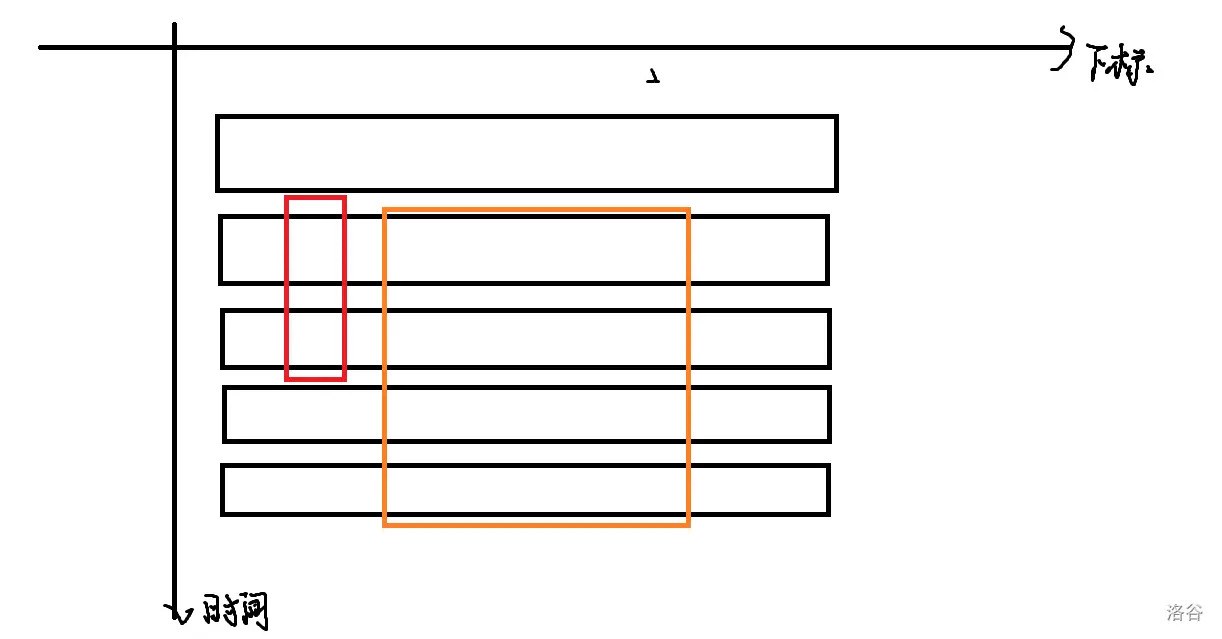
\includegraphics[width=10cm]{images/time.png}
\end{figure}
\par \noindent 把\textbf{初始数组按照时间轴赋值多份},于是最终认为:查询是查一个区间,但是修改是修改一个矩形(把当前时间到最后都会修改)。
~\\
\par \noindent 直接考虑离线询问,然后扫描线扫序列,然后数据结构维护时间维。
~\\
\par \noindent 考虑只有一个数的做法。 相当于要查询时间轴上有多少数 $≤K$ 
~\\
\par \noindent 离线然后按照时间分块,查询大块直接二分就行了(始终保持块内有序),散块暴力即可。

\begin{minted}{c++}
#include <bits/stdc++.h>
#define int long long
using namespace std;


const int N = 2e6;
int n, siz = 360, bel, q, num, cnt, ans[N], a[N], pos[N], LL[N], RR[N];
struct update {
    int x, tim, val;
    friend bool operator<(update x, update y) {
        return (x.x != y.x) ? x.x < y.x : x.tim < y.tim;
    }
} q1[N];
struct ask {
    int x, tim, val, id;
    friend bool operator<(ask x, ask y) {
        return (x.x != y.x) ? x.x < y.x : x.tim < y.tim;
    }
} q2[N];
int s[N], t[N], tag[N];
// t[] 维护块内有序
void rebuild(int L, int R) {
    for (int i = L; i <= R; i++) t[i] = s[i];
    sort(t + L, t + R + 1, greater<int>());
}
void change(int l, int r, int k) {
    l = max(l, 0ll);
    r = min(r, q);
    int pl = pos[l], pr = pos[r];
    if (pl == pr) {
        for (int i = l; i <= r; i++) s[i] += k;
        rebuild(LL[pl], RR[pl]);
        return;
    }
    // 大块懒标记
    for (int i = pl + 1; i <= pr - 1; i++) tag[i] += k;
    // 小块暴力 记得重构使得大块有序
    for (int i = l; i <= RR[pl]; i++) s[i] += k;
    rebuild(LL[pl], RR[pl]);
    
    for (int i = LL[pr]; i <= r; i++) s[i] += k;
    rebuild(LL[pl], RR[pl]);
}
int query(int l, int r, int k) {
    int pl = pos[l], pr = pos[r], cnt = 0;
    if (pl == pr) {
        for (int i = l; i <= r; i++)
            if (s[i] + tag[pl] >= k)
                cnt++;
        return cnt;
    }
    // 大块每块是有序的 二分求
    for (int i = pl + 1; i <= pr - 1; i++) {
        int l1 = LL[i], r1 = RR[i];
        while (l1 < r1) {
            int mid = l1 + r1 + 1 >> 1 ;
            if (t[mid] + tag[i] >= k)
                l1 = mid;
            else
                r1 = mid - 1;
        }
        if (t[l1] + tag[i] >= k) cnt += l1 - LL[i] + 1;
    }
    int L = LL[pr], R = RR[pl];
    for (int i = l; i <= R; i++) if (s[i] + tag[pl] >= k) cnt++;
    for (int i = L; i <= r; i++) if (s[i] + tag[pr] >= k) cnt++;
    return cnt;
}
signed main() {
    cin >> n >> q;
    for (int i = 1; i <= n; i++) cin >> a[i];
    for (int i = 1; i <= q; i++) {
        int op, l, r, x;
        cin >> op;
        if (op == 1) {
            cin >> l >> r >> x;
            q1[++cnt] = {l, i, x};
            q1[++cnt] = {r + 1, i, -x};
        }  else {
            cin >> l >> x;
            q2[++num] = {l, i, x, num};
        }
    }

    bel = (q + 1 - 1) / siz + 1;
    for (int i = 1; i <= bel; i++) {
        LL[i] = (i - 1) * siz + 1;
        RR[i] = min(i * siz, q + 1);
        for (int j = LL[i]; j <= RR[i]; j++) {
            pos[j] = i;
        }
    }
    //======================================= 时间轴分块
    sort(q1 + 1, q1 + cnt + 1);
    sort(q2 + 1, q2 + num + 1);
    memset(ans, -1, sizeof(ans));

    for (int i = 1, j = 1; i <= num; i++) {
        while ((q1[j].x < q2[i].x || (q1[j].x == q2[i].x && q1[j].tim < q2[i].tim)) && j <= cnt) {
            change(q1[j].tim + 1, q + 1, q1[j].val); // 不包括这一秒 在下一秒生效
            ++j;
        }
        ans[q2[i].id] = query(1, q2[i].tim, q2[i].val - a[q2[i].x]);
    }
    for (int i = 1; i <= q; i++)  if (ans[i] != -1) cout << ans[i] << "\n";
    return 0;
}
\end{minted}
